
%(BEGIN_QUESTION)
% Copyright 2006, Tony R. Kuphaldt, released under the Creative Commons Attribution License (v 1.0)
% This means you may do almost anything with this work of mine, so long as you give me proper credit

Bestem LRV- og URV-punktene for en transmitter som måler vannnivå i denne tanken, der $\Delta$P-transmitteren er montert 10 fot over tankbunnen og koblet med kapillarrør og fjernforsegling fylt med silikonfyllevæske (SG = 0.934):

$$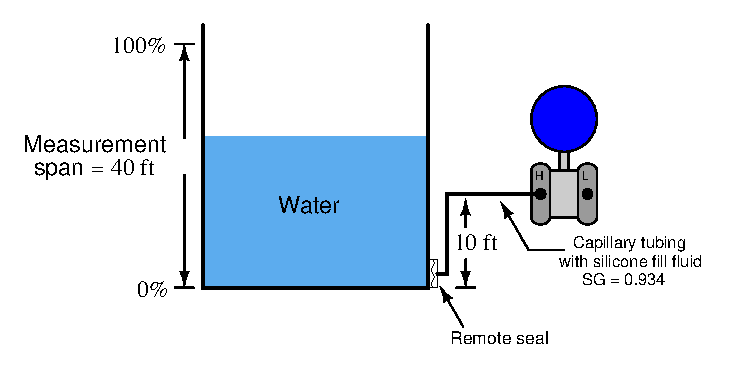
\includegraphics[width=15.5cm]{i00260x01.eps}$$

Forklar også hvorfor fjernforsegling er helt nødvendig i denne installasjonen.  Det ville ikke vært lurt å koble ``high''-porten på $\Delta$P-transmitteren direkte til tankbunnen med en rørslange, slik man kan når transmitteren står på nivå med tankbunnen eller under denne.

\vskip 10pt

Vis alt matematisk arbeid slik at instruktøren kan kontrollere den konseptuelle gyldigheten av metoden(e) dine.  En god kontroll er å verifisere at alle mellomregninger har fysisk mening.  {\bf Hvis du virkelig forstår hva du gjør, vil du kunne identifisere korrekt måleenhet for hvert mellomresultat og også vise hvor tallet gjelder i scenariet}.


\vskip 20pt \vbox{\hrule \hbox{\strut \vrule{} {\bf Forslag til sokratisk diskusjon} \vrule} \hrule}

\begin{itemize}
\item{} Demonstrer hvordan man kan {\it estimere} numeriske svar uten kalkulator.
\item{} Ved beregning av hydrostatisk trykk finnes to vanlige metoder: bruke formelen $P = \gamma h$, eller oversette tommer vertikal væskehøyde direkte til PSI via kjent sammenheng mellom vann og PSI (1 PSI = 27.68 inches water).  Demonstrer begge metodene på denne oppgaven.
\item{} En god problemløsningsmetode er tankeeksperiment med motsatt tilfelle.  Her ble du bedt om å forklare hvorfor fjernforsegling er nødvendig.  Presenter et tankeeksperiment der fjernforsegling mangler, og forklar hvordan dette hjelper deg å svare på hovedspørsmålet.
\item{} Bør ``low''-siden av DP-transmitteren ventileres eller forsegles?
\end{itemize}

\underbar{file i00260}
%(END_QUESTION)





%(BEGIN_ANSWER)

%(END_ANSWER)





%(BEGIN_NOTES)

Beregning av hydrostatisk trykk fra 10 fot kapillarrør (alene) under transmitteren:

$$\left(-10 \hbox{ ft silicone} \over 1 \right) \left(12 \hbox{ in} \over 1 \hbox{ ft} \right) \left(1 \hbox{ PSI} \over 27.68 \hbox{ in WC} \right) \left(0.934 \hbox{ in WC} \over 1 \hbox{ in silicone} \right) = -4.049 \hbox{ PSI}$$

\vskip 10pt

Full tank med vann gir ytterligere 40 fot hydrostatisk trykk på transmitterens ``H''-port:

$$\left(40 \hbox{ ft WC} \over 1 \right) \left(12 \hbox{ in} \over 1 \hbox{ ft} \right) \left(1 \hbox{ PSI} \over 27.68 \hbox{ in WC} \right) = 17.341 \hbox{ PSI}$$

\vskip 10pt

Når tanken er tom (LRV), ser transmitteren bare vakuumet på $-4.049$ PSI fra $-10$ fot silikonfyllevæske.  Når tanken er full (URV), ser transmitteren $-4.049$ PSI {\it pluss} 17.341 PSI fra 40 fot vann, totalt 13.292 PSI.

\vskip 10pt

LRV = $-112.08$ "W.C. = $-4.049$ PSI

\vskip 10pt

URV = +367.92 "W.C. = 13.292 PSI

\vskip 10pt

Hvis fjernforsegling mangler, kan væske i impulsledningen renne ut når nivået er lavt.  Da endres statisk trykk i impulsledningen, og nullpunktet (LRV) forskyves.

\vskip 10pt

Vi kan simulere vakuumtilstanden ved å legge positivt testtrykk på 112.08 "W.C. på {\it low}-porten av $\Delta$P-transmitteren.

%INDEX% Measurement, level: hydrostatic pressure (elevated zero)

%(END_NOTES)
